%% ----------------------------------------------------------------
%% Introduction.tex
%% ---------------------------------------------------------------- 
\chapter{Introduction} \label{Chapter:Introduction}
%The Introduction to my Report \dots

%The initial idea of the project was taken from Pirobot(\cite{Pirobot}).
%
%\inote{what it will do. Define everything. Use. Very general}
%General - mapping robots. 
%
%stereovision - uses etc.
%
%other similar projects
%
%why mine is important 


This report documents the design, test and build of a stereoscopic mapping robot. The end product will be a small, two wheeled robot with a roller ball, that will autonomously search and map an unkown area and build up an occupancy map of the searched area. 

Stereoscopy in computer vision is the ability of to calculate the locations and depths with ``images from two cameras are used to triangulate and estimate distances" (\cite{Saxena:DepthEstimation}). By using two cameras on the same plane and serparated by a set horizontal distance, depth of the observed scene can be perceived by the system.
\inote{Cite Occupancy Map}
An Occupancy map is a representation of an area where a location is given a value of either \textit{free, occupied} or \textit{unkown}.  Three dimensional occupancy maps can also be generated, such as the OctoMap (\cite{octomap}) and objects can also be tracked using an occupancy map and statistics (\cite{Fleuret:OccupancyMap}). 

The purpose of a mapping robot is to build a representation of the area around it. This then leads on to be able to conduct an application that requires knowledge of the area. One algorithm used to build up the occupancy map is the S.L.A.M. algorithm (\cite{Thrun:SLAM}) and is used in \cite{Se:MappingRobot}. Accurate mapping robots tend to used laser range finders (\cite{Ruhnke:LaserMapping}).

Stereovision is a small section of computer vision which is widely used in many applications, including Microsofts Xbox Kinect (\cite{Microsoft:Kinect}) where stereo vision is used to locate a game player to involve them more in the game. \cite{Mrovlje:Distance_Stereoscopic} uses stereovision to be able to locate the distance to a marker.

The stereovision mapping robot discussed in this report is a low cost alternative to other robots which use laser range finders or high quality cameras (\cite{Se:MappingRobot}). The robot discussed will use the base seen in figure \ref{fig:RobotBase} and use two OmniVision OV7670 cameras delivering up to VGA format images.

\begin{figure}
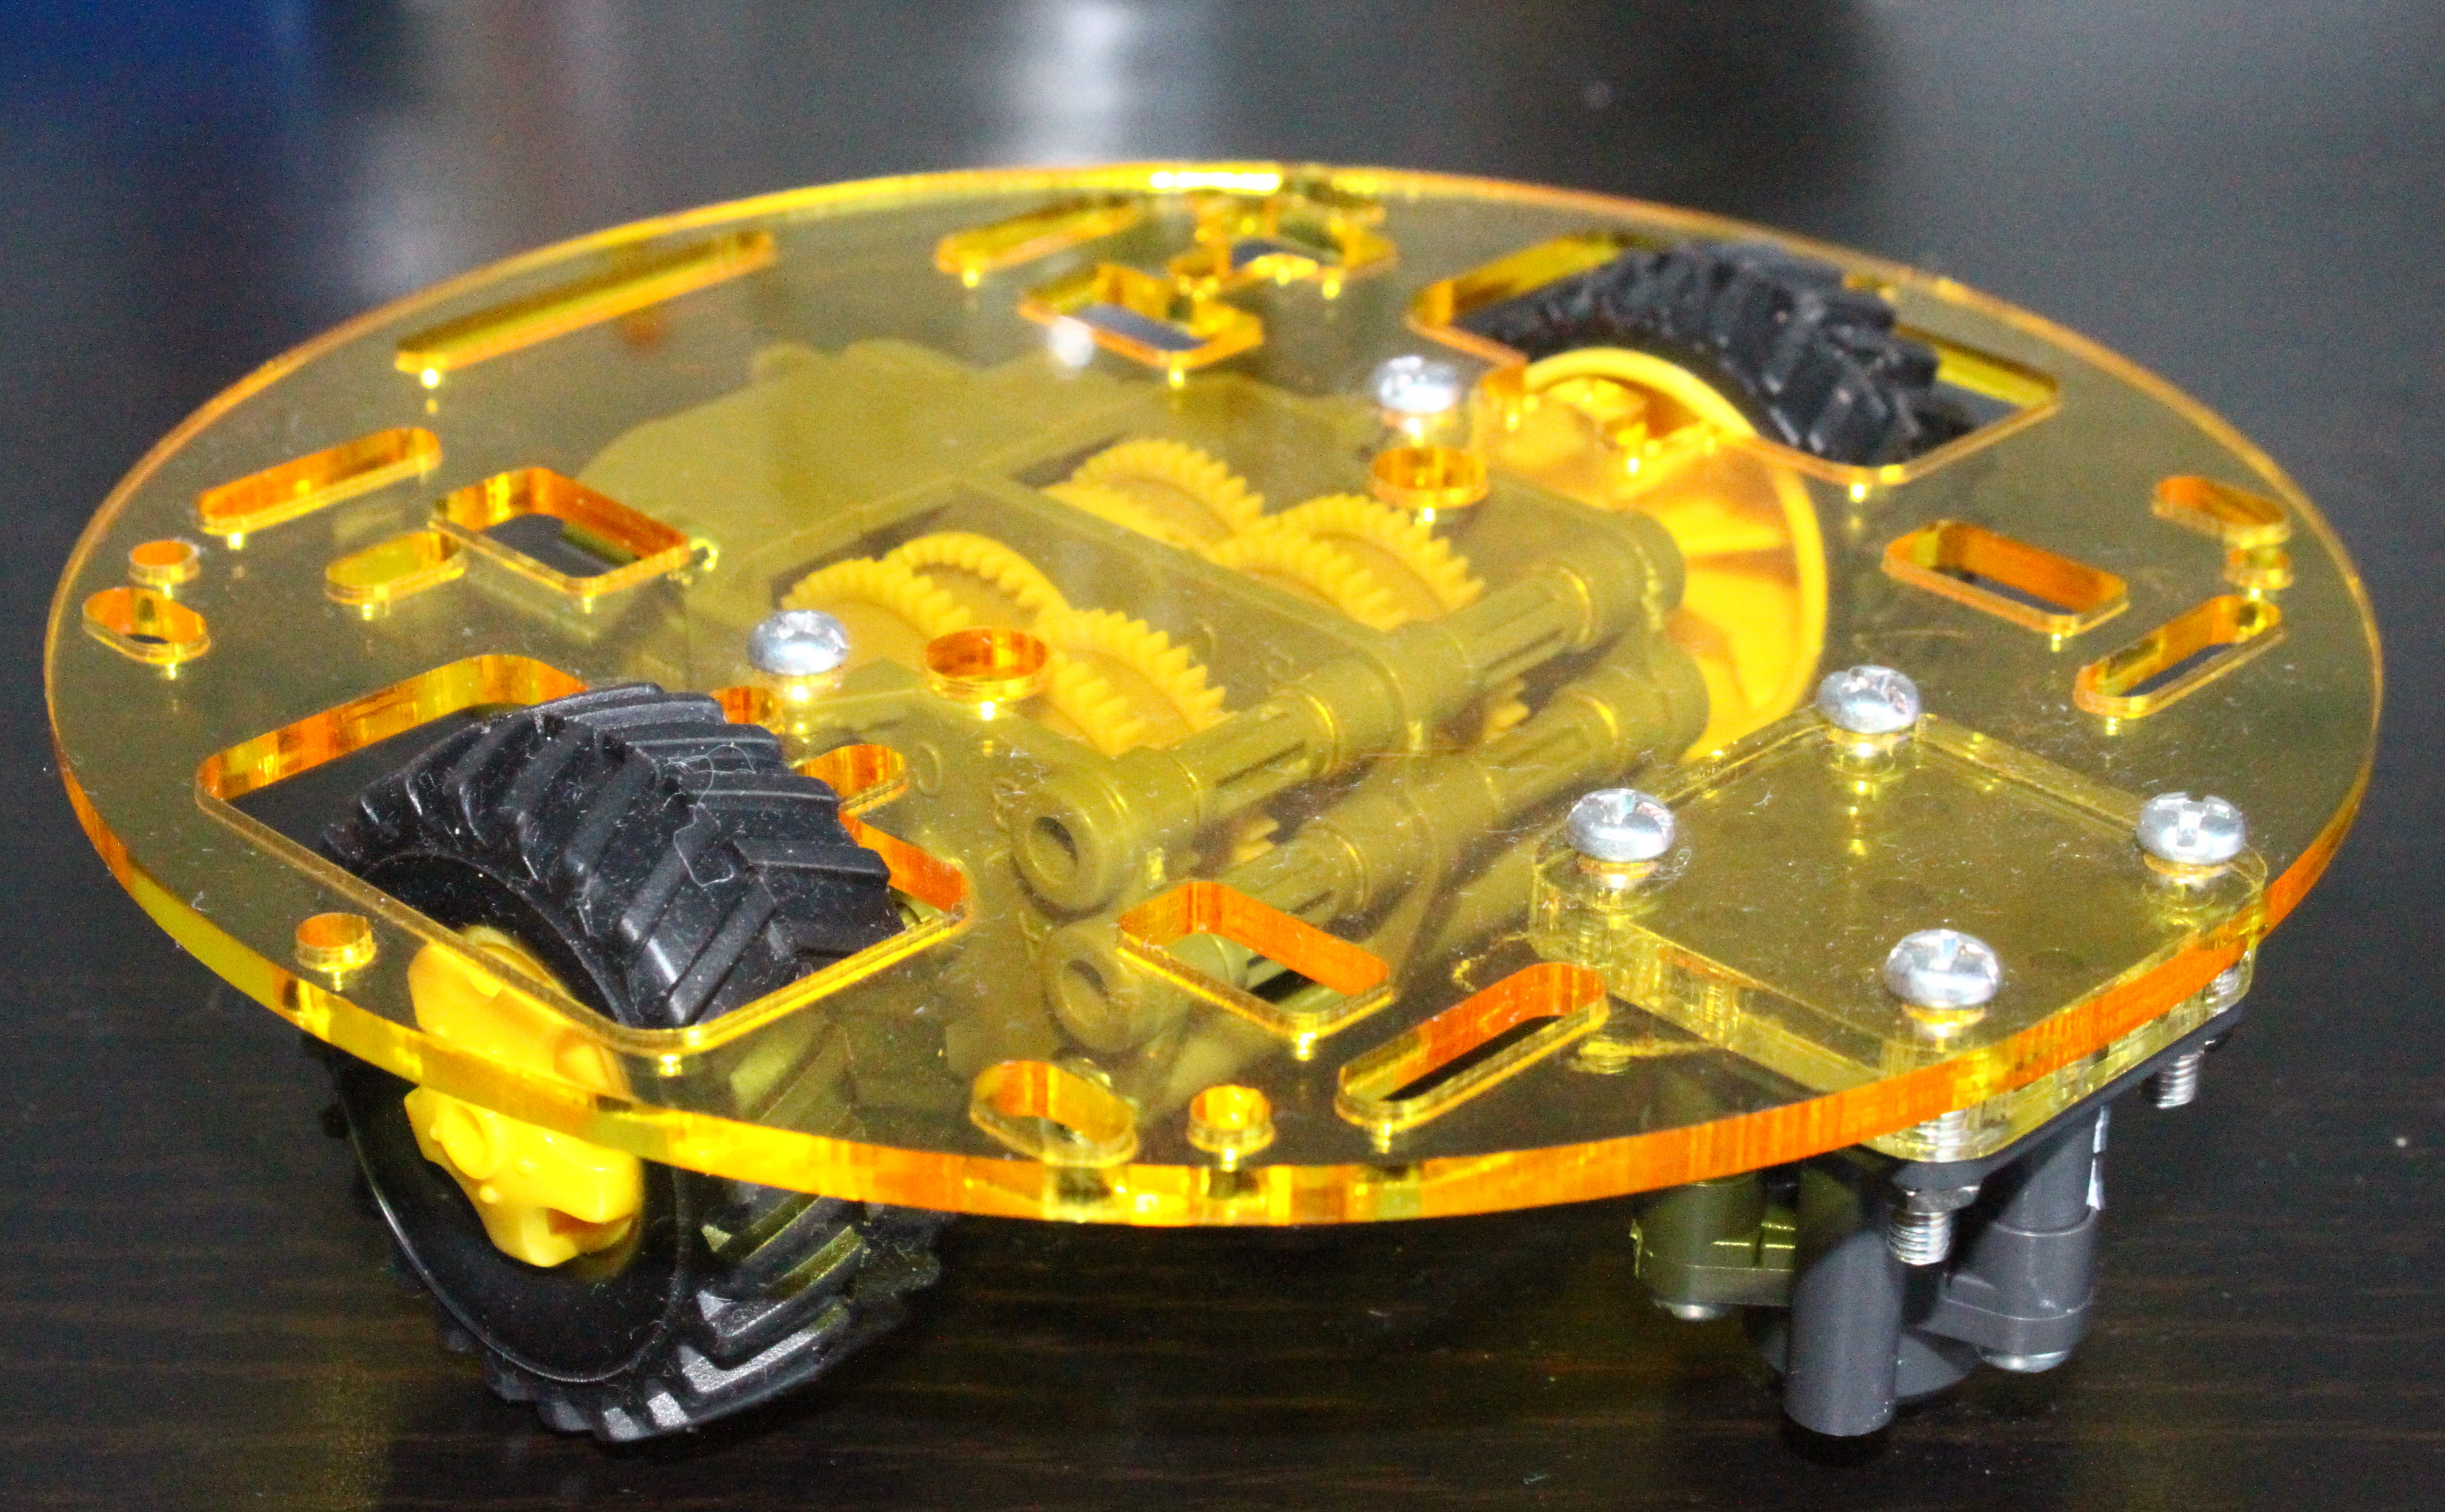
\includegraphics[width=\textwidth]{./Figures/RobotBase.jpg}
\caption{The base of the robot will use}
\label{fig:RobotBase}
\end{figure}